\documentclass[11pt]{scrartcl}
\usepackage[sexy]{evan}
\usepackage{graphicx}
\usepackage[spanish]{babel}
\graphicspath{ {./images/} }

\usepackage{answers}
\Newassociation{hint}{hintitem}{all-hints}
\renewcommand{\solutionextension}{out}
\renewenvironment{hintitem}[1]{\item[\bfseries #1.]}{}

\usepackage{venndiagram,multicol,hyperref,graphicx,array,xskak}

\begin{document}
\title{Grafos I}
\author{Ricardo Largaespada}
\date{18 y 25 Mayo 2024}

\maketitle
\section{Introducción}
\textit{¿Qué es un grafo?} Si nunca has oído hablar de esto antes, seguramente te estarás haciendo esta pregunta. Vamos a intentar satisfacer tu curiosidad contando cómo surgió la teoría de los grafos.\\

\begin{figure}[h]
    \centering
    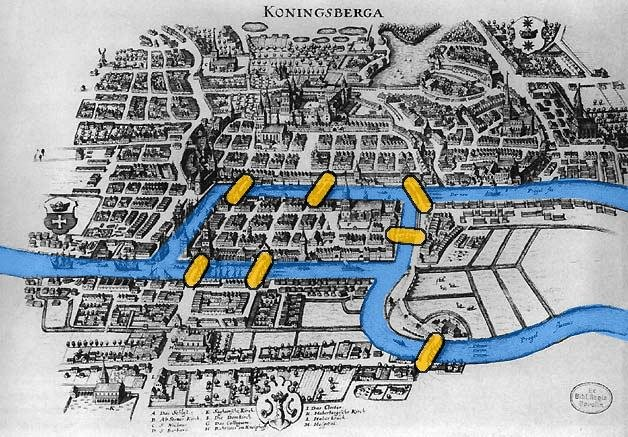
\includegraphics[scale=0.25]{images/clase_10_Mapa-de-1652-de-la-Ciudad-de-Koenigsberg-2-con-el-agua-y-los-puentes-resaltados.png}
    \caption{Mapa de Königsberg}
    \label{fig:1}
\end{figure}

La literatura afirma que la teoría de los grafos comenzó en la ciudad de Königsberg en 1736 por el gran matemático suizo Leonhard Euler (1707-1783). La ciudad estaba atravesada por el río Pregel, que tenía dos islas (figura \ref{fig:1}). Como era muy complicado transportar cargas y personas en barco, se construyeron algunos puentes para facilitar este desplazamiento entre las islas y las dos orillas. Después de un tiempo, la gente empezó a preguntarse si era posible salir de su casa, cruzar cada puente exactamente una vez y volver a la seguridad de su hogar.

\begin{figure}[h!]
    \centering
    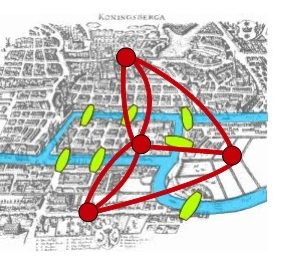
\includegraphics[scale=1]{images/clase_10_Konigs_Grafo.png}
    \caption{Diagrama de Euler}
    \label{fig:2}
\end{figure}

Para resolver el problema, Euler creó un diagrama que representaba el mapa de la ciudad. Lo hizo de la siguiente manera: a cada isla y orilla le asoció un punto que llamaremos \textit{ vértice} y a cada puente una conexión que llamaremos \textit{ arista}. Con esto, obtuvo la figura \ref{fig:2}.\\

Esta figura con varios puntos (vértices) y algunas conexiones (aristas) es lo que denominamos un \textit{ grafo}. Para finalizar su razonamiento, Euler se dio cuenta de que existían vértices con exactamente tres aristas incidentes. Por otro lado, como los habitantes querían cruzar cada puente solo una vez, cada vértice debería tener un número par de aristas. Por lo tanto, se tornaba imposible hacer un recorrido siguiendo las reglas impuestas por los habitantes.\\

Como en toda teoría matemática, la teoría de los grafos está llena de nomenclaturas y términos técnicos. En esta sección vamos a aprender algunas definiciones importantes para la comprensión completa de este capítulo. A continuación, damos un ejemplo de un grafo que representa un mapa de carreteras y ciudades.

\begin{center}
    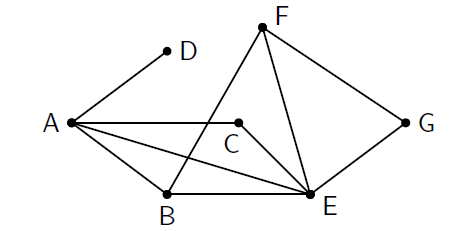
\includegraphics[scale=0.75]{images/clase_10_grafo_1.png}
\end{center}

Vamos a aprovechar el grafo anterior para abordar algunas definiciones. Por ejemplo, el grafo anterior es \textit{ conexo}, pues es posible ir de un vértice a cualquier otro usando algunas de sus aristas. Por ejemplo, para ir de A a G basta hacer la siguiente secuencia A $\rightarrow$ C $\rightarrow$ E $\rightarrow$ F $\rightarrow$ G. Decimos entonces que esta secuencia es un \textit{ camino} de A a G. Ahora, un camino cerrado se llama \textit{ ciclo}. Por ejemplo, el camino A $\rightarrow$ B $\rightarrow$ E $\rightarrow$ A es un ciclo de tamaño 3 (o sea, un $C_3$). Ya que el ciclo B $\rightarrow$ E $\rightarrow$ G $\rightarrow$ F $\rightarrow$ B es un $C_4$.\\

Otra notación muy importante es el \textit{ grado}. Vamos a definir el grado de un vértice $v$ como la cantidad de aristas que inciden en él. Y vamos a denotar esta cantidad como $d(v)$. Por ejemplo, $d(A) = 4$, $d(B) = 3$ y $d(C) = 2$. Los próximos ejercicios servirán para fijar las definiciones que acabamos de aprender.

\section{Ejercicios}
\begin{enumerate}
    \item Sabemos que el grafo anterior era conexo. Sin embargo, existe una arista que, si se retira, el grafo pasará a ser disconexo. ¿Cuál es esa arista? Explique por qué no puede ser otra.
    \item ¿Cuál es el camino más corto de D a C? ¿Y el más largo? (no se pueden repetir aristas)
    \item ¿Cuántos ciclos de tamaño tres existen? ¿Y de tamaño cuatro?
    \item Determine el ciclo que tiene el mayor tamaño.
    \item ¿Cuál es el vértice que tiene el mayor grado?
    \item Calcule la suma de los grados de todos los vértices del grafo.
\end{enumerate}

Debes haber notado que el grafo de Euler tiene una particularidad: entre el mismo par de vértices existen dos aristas que los unen. Sin embargo, la mayoría de los grafos que estudiamos son grafos simples. Es decir, grafos que no admiten lazos (aristas que comienzan y terminan en el mismo vértice) ni aristas múltiples (como en el grafo de Euler).\\

El próximo problema es uno de los más famosos problemas de toda la olimpiada de matemáticas. Puedes estar seguro de que aún oirás hablar de este problema muchas veces.

\begin{example}
¿Es posible que los caballos de la figura 1 estén en la posición de la figura 2?
\begin{minipage}{0.5\textwidth}
  \storechessboardstyle{3x3}{%
    maxfield=c3,
    showmover=false,
    showpos=false,
    clearboard
  }
  \chessboard[
    style=3x3,
    setpieces={na1,nc1,Na3,Nc3},
    padding=1ex,
  ]
  Figura 1
\end{minipage} \hfil\begin{minipage}{0.5\textwidth}
  \storechessboardstyle{3x3}{%
    maxfield=c3,
    showmover=false,
    showpos=false,
    clearboard
  }
  \chessboard[
    style=3x3,
    setpieces={na1,Nc1,Na3,nc3},
    padding=1ex,
  ]
  Figura 2
\end{minipage}
\end{example}
Solución. Vamos a enumerar las casillas del tablero de la siguiente forma:

\begin{center}
    7 \hspace{1cm} 8 \hspace{1cm} 9 \\
    4 \hspace{1cm} 5 \hspace{1cm} 6 \\
    1 \hspace{1cm} 2 \hspace{1cm} 3
\end{center}

Ahora vamos a construir un grafo con vértices 1, 2, ..., 9 donde vamos a unir dos vértices $i$ y $j$ si es posible que el caballo vaya de la casilla $i$ a la casilla $j$ usando solo un movimiento. De esta forma, obtenemos el siguiente grafo:

\begin{figure}[h!]
    \centering
    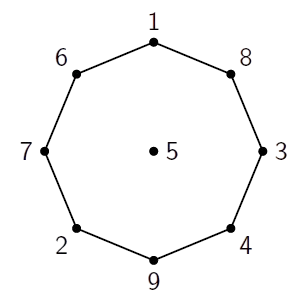
\includegraphics[scale=0.25]{images/clase_10_grafo_2.png}
    \caption{Grafo de los caballos}
\end{figure}

Ahora colocamos los caballos de acuerdo con los tableros mostrados anteriormente. Es fácil ver que es imposible ir de una configuración a otra, pues el orden cíclico de los caballos no puede cambiar, a menos que dos caballos estén sobre una misma casilla, y esto no es permitido.

\begin{theorem}
En un grafo simple $G = (V,A)$, la suma de los grados de todos sus vértices es igual al doble del número de aristas. Es decir:
\[
\sum_{v \in V} d(v) = 2|A|
\]
\end{theorem}
\begin{proof} De cada vértice $v$ parten $d(v)$ aristas. Sin embargo, cada arista tiene dos vértices. De este modo, si sumamos los grados de todos los vértices obtendremos el doble del número de aristas.\end{proof}

\begin{example}
Considere un grupo de 1997 personas. ¿Es posible que cada una de ellas conozca exactamente:
a) 3 personas?
b) 4 personas?
\end{example}
Solución. Primeramente, considere el grupo de 1997 personas como un grafo de 1997 vértices, en el que cada vértice representa a una persona. Y una arista une dos vértices si y solo si las dos personas asociadas son amigas.\\
Para el ítem (a) estamos suponiendo la existencia de un grafo cuya suma de todos los grados es $1997 \times 3$, es decir, un número impar. Esto es una contradicción, ya que la suma de todos los grados es igual al doble del número de aristas y, por lo tanto, un número par.\\

Para el ítem (b), considere un grafo cuyos vértices son $v_1, \ldots, v_{1997}$. Cada vértice $v_i$ está unido a los vértices $v_{i-2}$, $v_{i-1}$, $v_{i+1}$, $v_{i+2}$ para todo $i = 1, \ldots, 1997$. En que $v_{-1}=v_{1996}$, $v_{0}=v_{1997}$, $v_{1998}=v_1$ y $v_{1999}=v_2 $.\\

De todos los asuntos abordados por las matemáticas, la teoría de los grafos es de los que posee el mayor número de ideas diferentes. En esta sección vamos a resolver varios problemas de grafos usando estrategias que aprendimos anteriormente. Vamos a empezar demostrando un hecho conocido como teorema de Ramsey.

\begin{example}[Teorema de Ramsey]
    En un grupo de seis personas siempre existen tres que se conocen mutuamente o tres que no se conocen mutuamente.
\end{example}
Solución. Para resolver este problema vamos a usar el lenguaje de los grafos. De esta forma, piensa en un grafo con seis vértices $A, B, C, D, E, F$. Una arista continua representará una “amistad” y una arista punteada, una “enemistad”. Fijado el vértice $A$, sabemos que tiene cinco aristas. Como solo hay dos tipos de arista, uno de los tipos fue usado al menos tres veces. Sin pérdida de generalidad, supongamos que el tipo “continua” fue elegido tres veces.\\

\begin{center}
    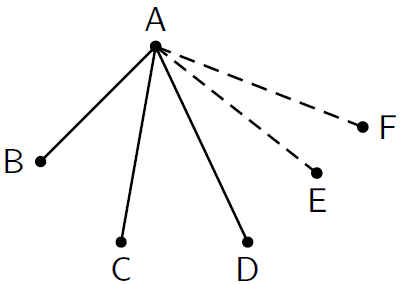
\includegraphics[scale=0.75]{images/clase_10_grafo_4.png}
\end{center}
Ahora, si una de las aristas $BC$, $CD$ o $DB$ es continua, tendremos tres personas conociéndose mutuamente. De lo contrario, las tres son punteadas. En este caso, $B, C$ y $D$ no se conocen mutuamente.\\

Ve que en el ejemplo anterior usamos esencialmente el principio del palomar. El próximo problema es de la olimpiada de Leningrado de 1990. En este ejemplo vamos a usar una idea un poco más sofisticada, el principio del extremo.

\begin{example}
    Florinia y Agrestia son países vecinos. Se sabe que cada ciudad está unida a un máximo de diez otras ciudades y que ciudades del mismo país no están unidas. Prueba que podemos pintar estas carreteras usando diez colores de modo que carreteras adyacentes tengan colores distintos.
\end{example}
Solución. Supongamos que inicialmente todas las carreteras están incoloras. Es claro que podemos elegir una de ellas y pintarla con uno de los colores. A partir de ahí vamos a pintar las demás carreteras respetando la siguiente regla:\\

Sean $X$ e $Y$ dos ciudades (una de cada país) tal que la carretera $XY$ está incolora. De este modo, existe un color (digamos el color 1) que no fue usado en ninguna de las carreteras que parten de $X$ y un color (digamos el color 2) que no fue usado en ninguna de las carreteras que parten de $Y$. Ahora elige el camino más largo de la forma $2-1-2-1-\cdots$ partiendo de $X$.
\begin{center}
    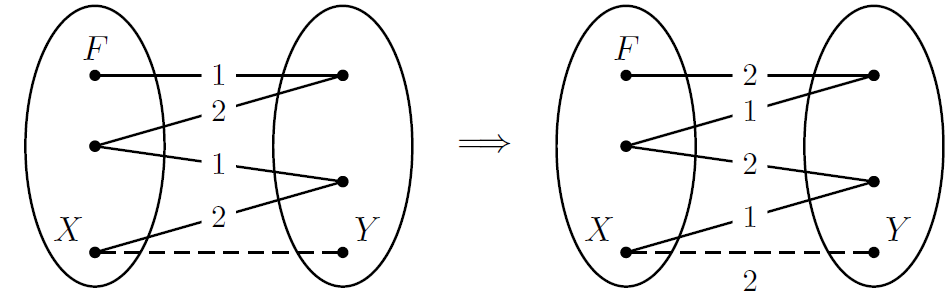
\includegraphics[scale=0.75]{images/clase_10_grafo_5.png}
\end{center}
Supongamos, sin pérdida de generalidad, que este camino termina en una arista de color 1 en la ciudad $F$. De este modo, no existe una carretera de color 2 partiendo de $F$. Con esto, podemos intercambiar los colores de las carreteras de este camino (donde sea 2 pintamos de 1 y viceversa) sin ningún problema. Para finalizar, basta pintar la carretera $XY$ del color 2.
\Opensolutionfile{all-hints}

\section{Problemas Propuestos}

\begin{problem}
Considere un grupo de 1998 personas. ¿Es posible que cada una de ellas conozca exactamente a 101 personas del grupo?
\end{problem}

\begin{problem}
Cada uno de los 102 estudiantes es amigo de al menos 68 otros alumnos. Prueba que existen cuatro estudiantes con el mismo número de amigos.
\end{problem}

\begin{problem}
Todos los vértices de un grafo tienen grado 3. Prueba que el grafo posee un ciclo.
\end{problem}

\begin{problem}
En un conjunto de \( n \) personas, en cualquier grupo de cuatro de ellas existe una que conoce a las otras tres. Prueba que existe una persona que conoce a todas las demás.
\end{problem}

\begin{problem}
La figura a continuación representa las conexiones viales entre 14 ciudades. ¿Existe un camino que pase por cada ciudad exactamente una vez?
\begin{center}
    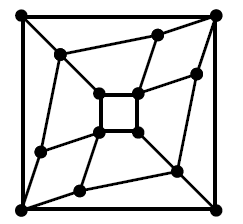
\includegraphics[scale=0.75]{images/clase_10_grafo_6.png}
\end{center}
\end{problem}

\begin{problem}
En un conjunto de \( 2n \) personas, cada una de ellas tiene un número par de amigos. Prueba que existen dos personas que tienen un número par de amigos en común.
\end{problem}

\begin{problem}
En Florinia, cualesquiera dos ciudades están conectadas por una carretera. Un emperador tirano decidió transformar todas estas carreteras en caminos de sentido único de tal forma que si una persona sale de su ciudad no podrá volver. ¿Es posible hacer tal crueldad?
\end{problem}

\begin{problem}
En un grafo \( G \) cada vértice tiene un grado de al menos 3. Prueba que en este grafo hay un ciclo con un número de aristas no divisible por 3.

\end{problem}

\begin{problem}
En cierto país existen más de 101 ciudades. La capital de este país está conectada por líneas aéreas a otras 100 ciudades, y cada ciudad, excepto la capital, está conectada a otras 10 ciudades (si \( A \) está conectado a \( B \), \( B \) está conectado a \( A \)). Además, todas las líneas aéreas son de una única dirección. Se sabe que de cualquier ciudad es posible llegar a cualquier otra usando estas rutas. Prueba que es posible cerrar la mitad de las líneas aéreas conectadas a la capital y preservar la capacidad de viajar de una ciudad a cualquier otra.
\end{problem}

\begin{problem}
En un torneo completo de tenis había 12 jugadores. Prueba que podemos encontrar tres jugadores \( A, B \) y \( C \) tales que \( A \) ganó a \( B \), \( B \) ganó a \( C \) y \( C \) ganó a \( A \).
\end{problem}

\begin{problem}
    Un grafo orientado tiene 1001 vértices. Cada vértice tiene 500 entradas y 500 salidas. Muestra que cualquier subgrafo de 668 vértices es conexo.
\end{problem}

\begin{problem}
    En un grupo de 50 científicos se sabe que cada uno de ellos conoce al menos a 25 otros científicos. Prueba que podemos colocar cuatro de ellos alrededor de una mesa de forma que cada científico esté sentado al lado de dos amigos.
\end{problem}

\begin{problem}
    En un país con seis ciudades cualesquiera dos están conectadas por una línea aérea (ida y vuelta). Cada línea aérea es operada por exactamente una de las dos empresas aéreas existentes. Muestra que existen cuatro ciudades \( A, B, C, D \) tales que las líneas \( AB, BC, CD, DA \) son controladas por una única empresa.
\end{problem}

\begin{problem}
    En un grafo de 17 vértices todas las aristas están trazadas y pintadas de uno de tres colores. Prueba que existe un triángulo con las tres aristas del mismo color.
\end{problem}

\begin{problem}
    En una sala hay nueve hombres. Se sabe que en cualquier grupo de tres de ellos existen dos que se conocen. Prueba que podemos elegir cuatro de ellos que se conocen mutuamente.
\end{problem}

\begin{problem}
    En un grupo de \( n \) personas se sabe que si dos tienen el mismo número de amigos, entonces no tienen amigos en común. Prueba que existe una persona con exactamente un amigo.
\end{problem}
\Closesolutionfile{all-hints}

%\section{Sugerencias y Soluciones}
%\begin{enumerate}
%\input{all-hints.out}
%\end{enumerate}

\end{document}